%%
%% This is file `sample-manuscript.tex',
%% generated with the docstrip utility.
%%
%% The original source files were:
%%
%% samples.dtx  (with options: `manuscript')
%% 
%% IMPORTANT NOTICE:
%% 
%% For the copyright see the source file.
%% 
%% Any modified versions of this file must be renamed
%% with new filenames distinct from sample-manuscript.tex.
%% 
%% For distribution of the original source see the terms
%% for copying and modification in the file samples.dtx.
%% 
%% This generated file may be distributed as long as the
%% original source files, as listed above, are part of the
%% same distribution. (The sources need not necessarily be
%% in the same archive or directory.)
%%
%% Commands for TeXCount
%TC:macro \cite [option:text,text]
%TC:macro \citep [option:text,text]
%TC:macro \citet [option:text,text]
%TC:envir table 0 1
%TC:envir table* 0 1
%TC:envir tabular [ignore] word
%TC:envir displaymath 0 word
%TC:envir math 0 word
%TC:envir comment 0 0
%%
%%
%% The first command in your LaTeX source must be the \documentclass command.
\documentclass[manuscript,screen,review]{acmart}
\usepackage{subcaption}

%%
%% \BibTeX command to typeset BibTeX logo in the docs
\AtBeginDocument{%
  \providecommand\BibTeX{{%
    \normalfont B\kern-0.5em{\scshape i\kern-0.25em b}\kern-0.8em\TeX}}}

%% Rights management information.  This information is sent to you
%% when you complete the rights form.  These commands have SAMPLE
%% values in them; it is your responsibility as an author to replace
%% the commands and values with those provided to you when you
%% complete the rights form.
\setcopyright{acmcopyright}
\copyrightyear{2022}
\acmYear{2022}
\acmDOI{XXXXXXX.XXXXXXX}

%% These commands are for a PROCEEDINGS abstract or paper.
% \acmConference[Conference acronym 'XX]{Make sure to enter the correct
%   conference title from your rights confirmation emai}{June 03--05,
%   2018}{Woodstock, NY}
% \acmPrice{15.00}
% \acmISBN{978-1-4503-XXXX-X/18/06}


%%
%% Submission ID.
%% Use this when submitting an article to a sponsored event. You'll
%% receive a unique submission ID from the organizers
%% of the event, and this ID should be used as the parameter to this command.
%%\acmSubmissionID{123-A56-BU3}

%%
%% For managing citations, it is recommended to use bibliography
%% files in BibTeX format.
%%
%% You can then either use BibTeX with the ACM-Reference-Format style,
%% or BibLaTeX with the acmnumeric or acmauthoryear sytles, that include
%% support for advanced citation of software artefact from the
%% biblatex-software package, also separately available on CTAN.
%%
%% Look at the sample-*-biblatex.tex files for templates showcasing
%% the biblatex styles.
%%

%%
%% The majority of ACM publications use numbered citations and
%% references.  The command \citestyle{authoryear} switches to the
%% "author year" style.
%%
%% If you are preparing content for an event
%% sponsored by ACM SIGGRAPH, you must use the "author year" style of
%% citations and references.
%% Uncommenting
%% the next command will enable that style.
%%\citestyle{acmauthoryear}

%%
%% end of the preamble, start of the body of the document source.
\begin{document}

%%
%% The "title" command has an optional parameter,
%% allowing the author to define a "short title" to be used in page headers.
\title{Jump Force: Democratizing Actionable Rehabilitation}

%%
%% The "author" command and its associated commands are used to define
%% the authors and their affiliations.
%% Of note is the shared affiliation of the first two authors, and the
%% "authornote" and "authornotemark" commands
%% used to denote shared contribution to the research.
\author{Joshua Schmidt}
\email{jns223@cornell.edu}
\affiliation{%
  \institution{Cornell Tech}
  \streetaddress{1 East Loop Rd}
  \city{New York City}
  \state{New York}
  \country{USA}
  \postcode{10044}
}

%%
%% By default, the full list of authors will be used in the page
%% headers. Often, this list is too long, and will overlap
%% other information printed in the page headers. This command allows
%% the author to define a more concise list
%% of authors' names for this purpose.
\renewcommand{\shortauthors}{Schmidt, et al.}

%%
%% The abstract is a short summary of the work to be presented in the
%% article.
\begin{abstract}
  Jump Force is a novel data collection device for automating and standardizing the vertical jump Return to Play protocol. This protocol is used today to assess the state of an athlete's rehabilitation when recovering from knee injuries, one of the most common injury types in the NCAA. This wearable device consists of an array of sensors used to analyze the angle, speed and other characteristics of vertical jumps, using this data to estimate the amount of force exerted over time. There is further discussion as to how to make this data more accessible, consistent and actionable, to reinvent the protocol.
\end{abstract}

%%
%% The code below is generated by the tool at http://dl.acm.org/ccs.cfm.
%% Please copy and paste the code instead of the example below.
%%
\begin{CCSXML}
<ccs2012>
   <concept>
       <concept_id>10003120.10003138.10003140</concept_id>
       <concept_desc>Human-centered computing~Ubiquitous and mobile computing systems and tools</concept_desc>
       <concept_significance>500</concept_significance>
       </concept>
 </ccs2012>
\end{CCSXML}

\ccsdesc[500]{Human-centered computing~Ubiquitous and mobile computing systems and tools}

%%
%% Keywords. The author(s) should pick words that accurately describe
%% the work being presented. Separate the keywords with commas.
\keywords{ubiquitous computing, actionable rehabilitation, data collection, return to play, wearable sensors, HCI, Ubiquitous Computing}


%%
%% This command processes the author and affiliation and title
%% information and builds the first part of the formatted document.
\maketitle

\section{Introduction} \label{sec:introduction}

According to the most recent estimates for 2021, among the more than 500,000 college athletes who competed in the NCAA there were more than 210,000 reported injuries, and more than 90\% of participants stated they had some form of injury \cite{dart_2021}. Some high profile players, such as Stanley Doughty (defensive lineman at the University of South Carolina) and Marcus Lattimore, also from USC, were forced to quit their sports due to serious injuries \cite{dart_2021}. These injuries vary widely in scope and areas of the body affected. The most common are head and ankle injuries \cite{Caplan2014}, with an average of 10,560 concussions \cite{doi:10.1177/0363546515599634} and 47,250 ankle injuries \cite{Tummala2018-gv} reported over the 2009-2010 and 2013-2014 seasons. Knee related injuries were the third most common, with 8,470 reported over the 2013-2014 season \cite{doi:10.1177/0363546515599634, Arendt1995-ze}. These numbers are getting worse, not better, as athletes take more risks and there is more inclusivity and competition in sports. Injuries overall are up 4.7\% in the 2021-2022 season compared to the 2013-2014 season \cite{dart_2021, doi:10.1177/0363546515599634}. There are even instances of injuries that are fatal.

The number of injuries per year is staggering, and it is troubling that the problem is getting worse, not better. However, with every major problem there are opportunities for novel solutions. Instead of looking at the all sports injuries or even all injuries in a given sport, it is necessary to reduce scope to an actionable level. In this paper, we will be exploring specifically knee-related injuries, and how novel data-collecting methods can help with preventing repeated injuries. We will focus on the return-to-play protocol, a system physical therapists use to gauge injury recovery. We will propose a novel data collection system, \textit{Jump Force}, that uses a smart knee pad to automate this protocol, and discuss future areas for work.

\subsection{Return to Play Protocol}

The term \textit{Return to Play Protocol} is used loosely in the sports industry and varies from sport to sport. It sometimes even varies between trained professionals. There were some recent attempts at standardizing the protocols by sport \cite{doi:10.1080/00913847.2017.1288544}, but these have not caught on yet. The \textit{Return to Play Protocol} is a test that trained physical therapists conduct to determine if an athlete is fit to play again. Typically the assessment includes testing muscular force by comparing complimentary muscle groups, i.e. left hand to right hand, right arm to left arm, right knee to left knee. Practitioners would assess functional gait abnormalities as the patient performs standard motions (wrist rotation, arm curl, jump) \cite{doi:10.1080/00913847.2017.1288544}.

This procedure is largely qualitative, comparing a healthy side to an injured side, and does not have a set baseline for expected results \cite{doi:10.1080/00913847.2017.1288544}. There is also typically no standard form of data collection, though there is some research in that field as well \cite{10.1093/arclin/18.3.293}. Another limitation of these procedures is they often need to be completed in a sterile environment, i.e. off the playing field, making it less accurate accessible to athletes who want to play as soon as possible \cite{doi:10.1080/00913847.2017.1288544}. Additionally, due to the limited time span of these procedures (on average 5-10 minutes), they are unable to measure fatigue and endurance accurately \cite{10.1093/arclin/18.3.293}. Any enhancement to the \textit{Return to Play Protocol} would need to address most if not all of these issues, while making it more accessible to those who should be tested.

\subsection{Vertical Jump Methods}

The \textit{Return to Play Protocol} variant we will be focusing on is the \textit{Vertical Jump} method. This variant is the most widely used for knee-related injuries due to its simplicity \cite{Petersen2013}. The method assesses the strength of the patient's glutes, quads, hamstring's and calves, and assesses their athletic power \cite{Petersen2013}. There are several different Vertical Jump test methods, including chalk on wall (jumping and marking how high you get), Vertec (a specialized vertical jump tester), and a pressure / force plate. In this experiment we are using a force plate test as our baseline \cite{Petersen2013}.

In the vertical jump, there are several different events. These include standing, crouching, takeoff, peak height, and landing \cite{Petersen2013}. These correspond to different stages: before the jump, descend, accelerate up, flight to peak, flight to landing, and after the jump \cite{Petersen2013}. See the figure \ref{fig:jump_phases} below. 

% TODO - fix all pictures

\begin{figure}[ht]
  \centering
  \includegraphics[width=\linewidth]{images/jump_phases.png}
  \caption{Vertical Jump Phases.}
  \Description{Set of phases occurring in a given vertical jump test.}
  \label{fig:jump_phases}
\end{figure}

In this protocol, we are most concerned with how the force created from the descend and accelerate up events translates to the maximum height of the jump. Athletes that have equal force to height ratios before and after injuries, after several subsequent tests, are fit to return to play. Ideally, we will compare the athletes to a baseline that they recorded before their injury occurred, and one that is recent enough to reflect their athletic ability.

\section{Design}

When initially designing \textit{Jump Force}, the goal was to create a device that contains enough sensors to fully explain the motion of the jump. We wanted the device to be small enough to fit in a standard knee pad, and not require any external specialized equipment. To determine the height of the jump, we opted for camera vision, using the camera included in your smartphone. The types of sensors we added to analyze the motion of the jump include flex sensors, hall effect sensors, and accelerometers. Below is a figure \ref{fig:initial_design} of the initial design.

\begin{figure}[ht]
  \centering
  \includegraphics[width=0.5\linewidth]{images/initial_design.png}
  \caption{Initial design.}
  \Description{Initial design of \textit{Jump Force}, using two hall effect sensors}
  \label{fig:initial_design}
\end{figure}

\subsection{Sensors}

There were two types of \textit{Spectra} flex sensors used, single-sided and double sided, in pairs of two, one of both sides of the kneecap. This creates a matrix of four flex sensors. The \textit{US1881} hall effect sensor was placed at the top of the knee pad, with a neodymium magnet placed on the opposite end of the knee pad. The distance between the magnet and hall effect sensor is a constant, at 10.5cm, and with the distance to the rotation axis also known (5.25cm), it is straightforward to determine the angle of the knee at any given time. The flex sensors are used individually to calculate the current angle. Once calibrated, they generate a voltage when deformed which linearly correlates to the amount of deformation. This information can be used to find the current bend angle of the knee during the jump.

One goal of this experiment was to find the combination of sensors that would show the most accurate representation of the angle of the knee over time, and how that correlates to force exerted over time. That is why we included both flex sensors and hall effect sensors. There was only one hall effect sensor in the final design, but in the initial there were two for redundancy. The reason why we excluded one of the hall effect sensors was when testing we saw that it was not necessary. The hall effect sensors produced near identical results. However, we found that the flex sensors were not nearly as accurate, producing $8\%-15\%$ deviations in values between trials. This was after calibration steps. Aggregating the results from multiple flex sensors did help to smooth out this noise, lowering the deviation to $4\%-8\%$.

\subsection{Hall Effect Sensor Placement}

After deciding to use only a single Hall Effect sensor, the next question was how it would be mounted. At first, it was mounted in the front of the knee pad, so the sensor would be closer to the microcontroller collecting the data. However after conducting preliminary tests we noticed that the amount of mass between the sensor and magnet adds too much noise to the signal. Instead placing the sensor on the inside of the kneepad enables the sensor and magnet to have a direct line of sight, and therefore has a much cleaner signal. Compared to the old configuration, placing the Hall Effect sensor on the back of the knee pad increased accuracy by $68\%$.

\subsection{Microcontroller}

In order to collect all of this sensor data, we used a Heltec ESP-32 WiFi v2 microcontroller \cite{heltec-wifi-kit-32}. This controller uses a dual core 240MHz Tensilica LX6 chip with onboard WiFi and Bluetooth 5, and has an onboard 12-bit ADC. $47.5 k\Omega$ ballast resistors are added to the circuit before connecting the flex sensors to the ADC. In addition to the flex sensors and hall effect sensor, the microcontroller is connected to a 9DoF BNO055 IMU \cite{imu-BNO055}. This IMU is used for collecting acceleration data to more directly correlate the jump motion to force exerted, when doing the \textit{Return to Play Protocol}.

All of this sensor data is sampled at 120Hz. This sampling rate was chosen because it is twice the frame rate of the camera on modern-day smartphones, which is used for getting the height of the jump. Several filters were used to process the data before it left the microcontroller. These filters include a bandpass filter for the flex sensors and a lowpass filter for the hall effect sensor. Each of the flex sensor filters and hall effect sensor filter needed to be individually calibrated experimentally. These filters helped increase the accuracy of the sensor system dramatically, as the initial data was too noisy to be useful. Once the basic filtering is done it is ready to be processed.

\subsection{Smartphone Connection}

The Bluetooth protocol is used to get the data off of the microcontroller. Users can connect to the kneepad (the microcontroller) using a custom mobile app, and as soon as they connect they can start the recording process. A screenshot of the app is shown in the below figures \ref{fig:app_screens_1}.

\begin{figure}[ht]
  \centering
  \begin{subfigure}{0.5\textwidth}
    \centering
    \includegraphics[width=0.55\linewidth]{images/connect_screen.jpg}
    \caption{Connect Screen.}
    \Description{Connect screen for \textit{Jump Force} mobile app.}
    \label{fig:app_screens_1}
  \end{subfigure}
\end{figure}

The mobile app is written using React Native \cite{react-native} and Expo \cite{expo-documentation}, allowing fast iteration of designs and user interface. NativeBase was the component library used to allow for native styling on both Android and iOS devices \cite{nativebase}.

\subsection{Initial Cloud Processing}

After you finish recording both the video file and kneepad data is uploaded to an AWS S3 bucket. The kneepad data is saved as a csv file, with all of timestamps recorded in ISO8601 format. Uploading triggers an AWS Lambda function to analyze the video file. This function uses the OpenCV python library \cite{opencv} to track the movement of green markers on the kneepad. Using the known distance between the camera and the kneepad of 2.5 meters, the function calculates the height at all of the timestamps in the kneepad data file. Since the kneepad is sampling at twice the speed of the camera, the height information for a given frame is generally mapped to two samples. After this lambda function is finished, the data is saved to a concatenated csv file in S3 containing all of the kneepad fields plus the height at that time.

Saving the concatenated csv file triggers a second lambda function, the data processing function. This function analyzes the flex sensor, hall effect, IMU and height data, and correlates it with the ground-truth force data, the data from the force plate. This force plate data is collected on a laptop using a simple python script with a serial logger, which generates a csv file and saves it to the same S3 bucket. The force plate data is sampled at 9600 baud or 9.6kHz, which is more than fast enough to support the kneepad data rate of 120Hz. The force plate is from Vernier, and you can find technical specifications here \cite{force-plate}. A picture of the force plate is shown below \ref{fig:force_plate}.

\begin{figure}[ht]
  \centering
  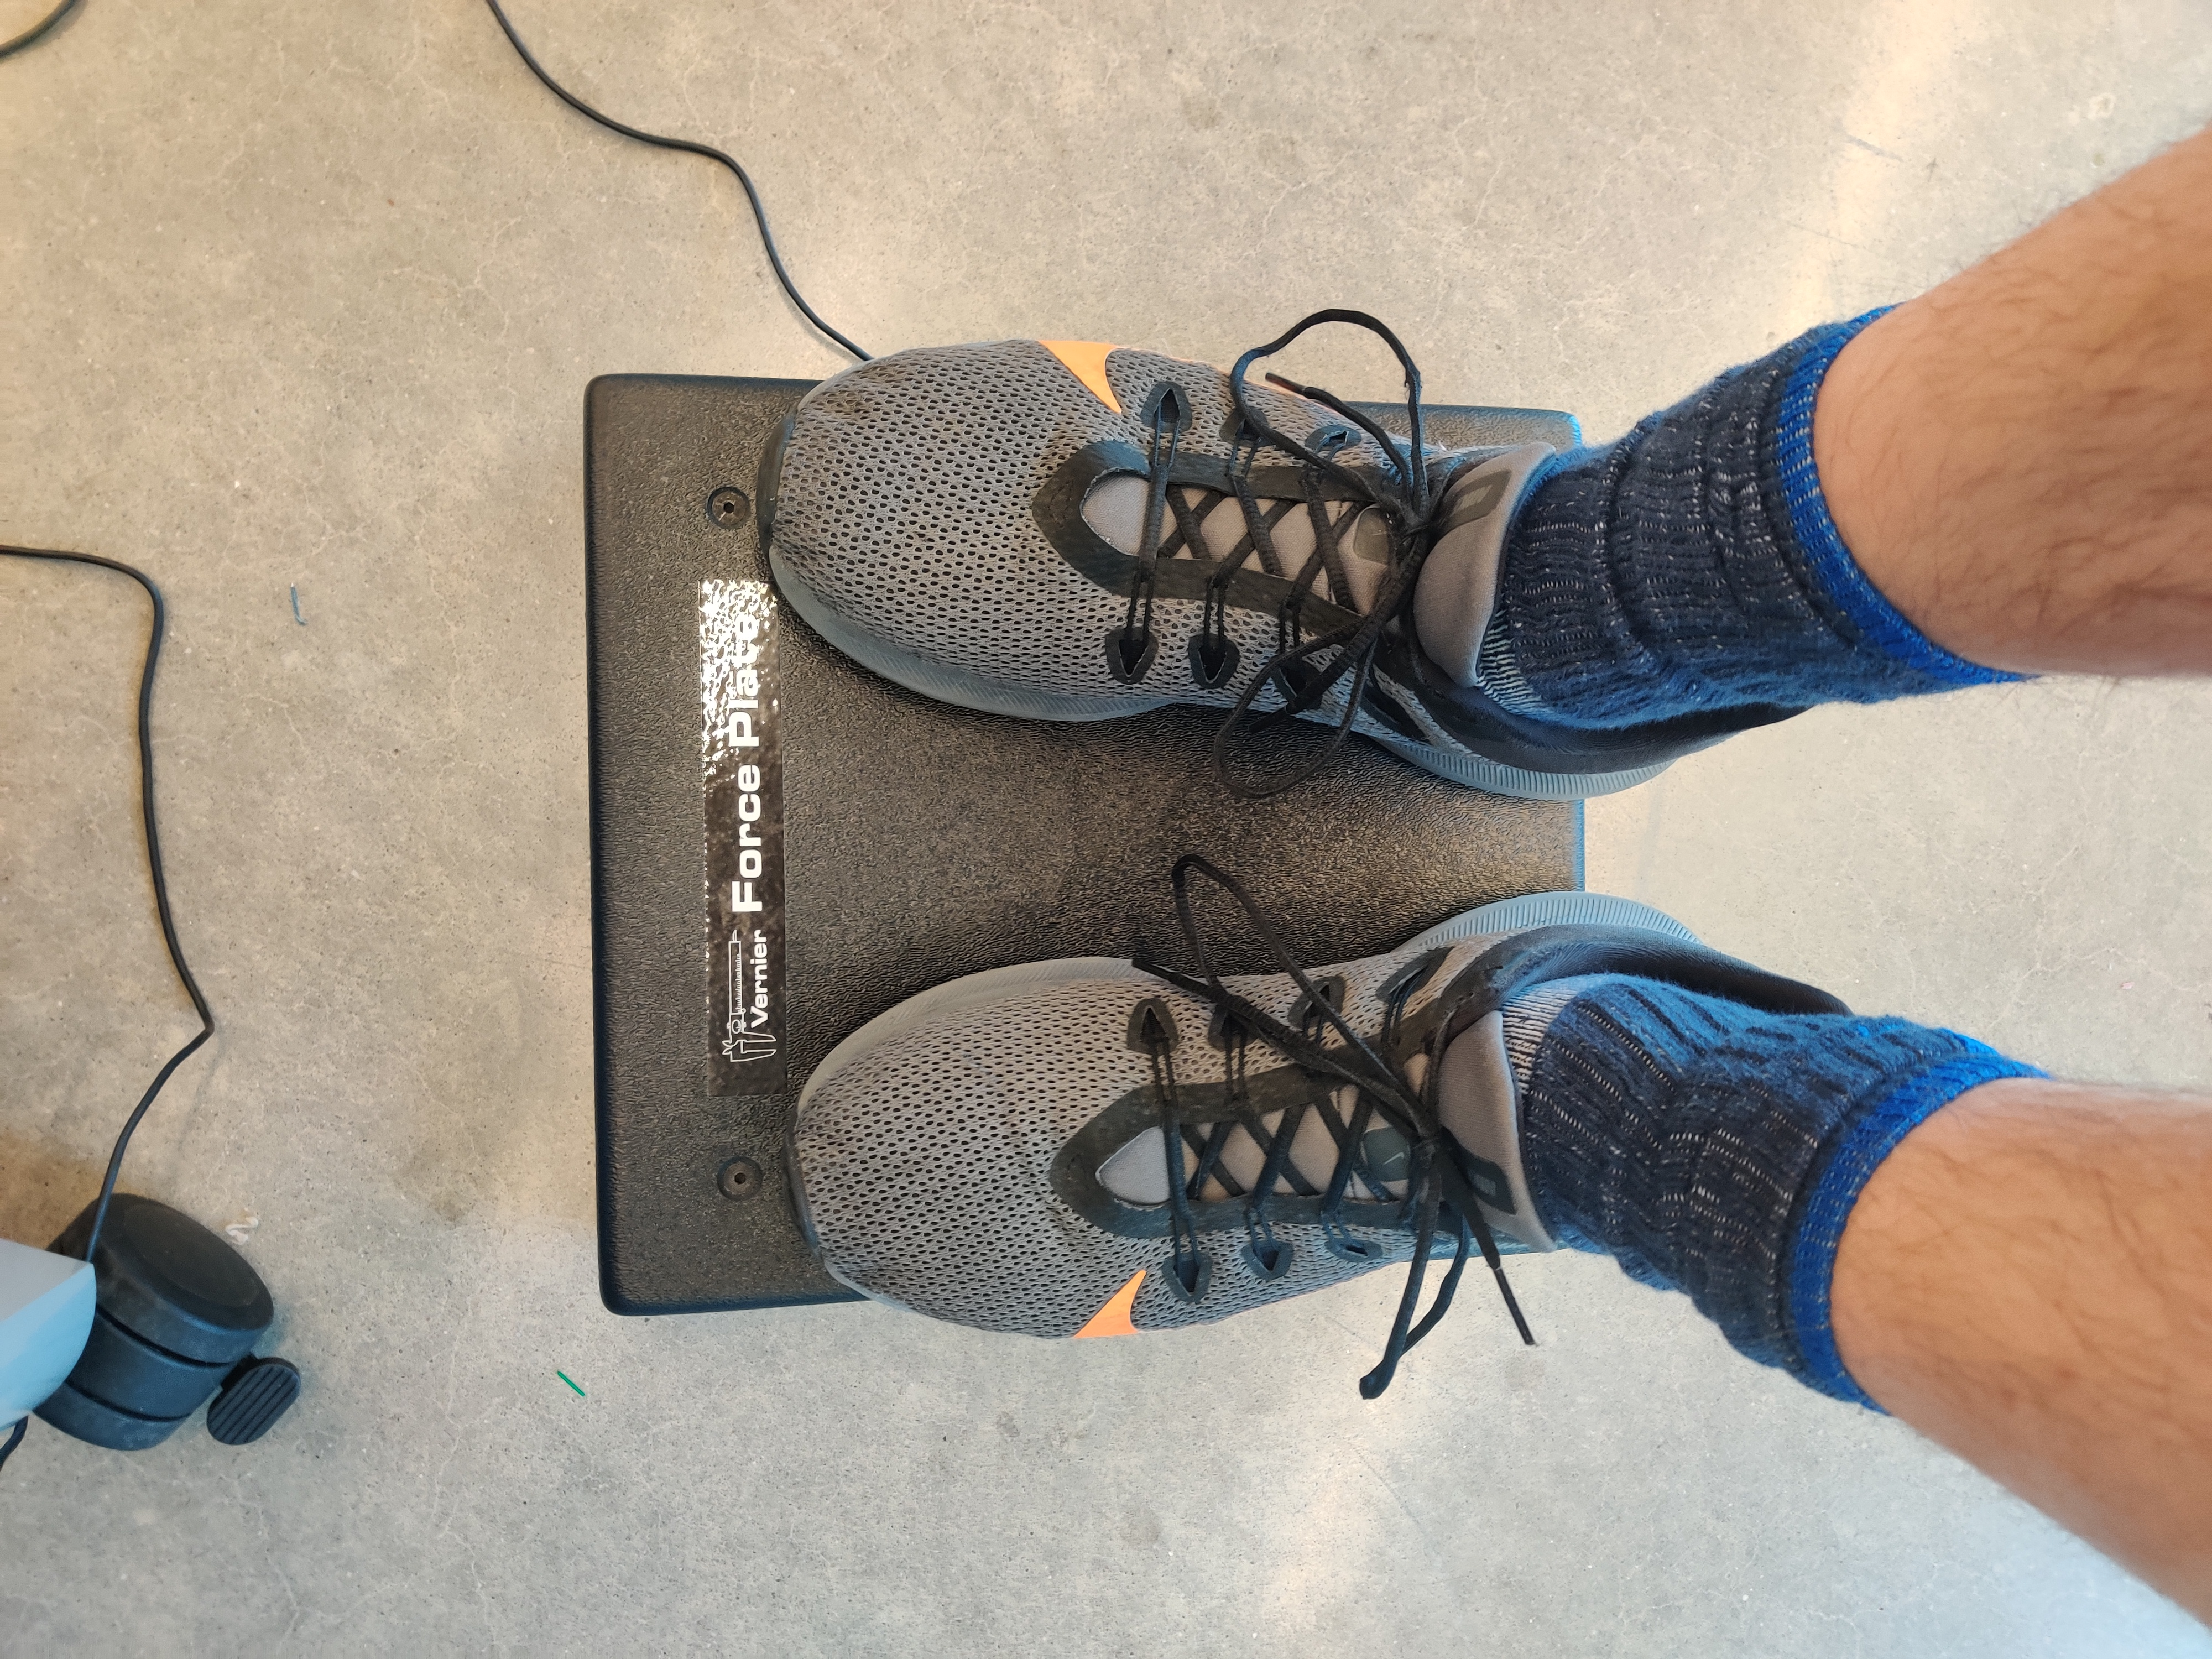
\includegraphics[width=0.5\linewidth]{images/force_plate.jpg}
  \caption{Force Plate.}
  \Description{Vernier force plate in experiment.}
  \label{fig:force_plate}
\end{figure}

\subsection{Force Correlation Processing}

The data processing function finds the angle the knee is bent in at any given time, and calculates the bend rate in the \textit{descend} and \textit{accelerate up} phases. With this data, we are able to calculate the correlation between bend rate and force exerted, and between initial acceleration and force exerted. This data can be found in the Results \ref{sec:results} section. We were also able to break out the bend rate correlations into data from each sensor type (hall effect and flex sensors). Jump height and acceleration data are also added as normalization factors for the knee angle, to test if this improves the correlation between the force exerted and knee angle.

\section{Experimental Procedure}

The Experimental Procedure is as follows. We record ten jumps at a time, with participants told to try to make the jump height and style as consistent as possible. We told participants to try to only use their knees to jump, as opposed to their ankles or muscle groups besides their quads.

\subsection{Questionnaire} \label{sec:questionnaire}

We have participants fill out a simple questionnaire containing questions such as how many times and for what duration the participant exercises per week, if they are involved in any sports and if so, which ones, how they would rate their athletic abilities, the longest distance they are able to run, and how high do they think they are able to jump. All of this data is used to control for different athletic abilities in the experimental results, and gain a more qualitative understanding of our participants.

\subsection{Procedure} \label{sec:procedure}

Participants do the set of ten jumps three times, for a total of 30 jumps, with a one minute break in between each set. This makes the total time for the experiment less than 10 minutes per participant, from start to finish. The jumps are conducted in a controlled environment indoors, on a force plate, when wearing the Jump Force kneepad. This is the only environment in which we are able to conduct this experiment, because the force plate would be less accurate on an actual soccer field. After doing the jumps they complete the exit survey as described here \ref{sec:questionnaire}, and additionally submit feedback as to the quality of the experiment.

\subsection{Prototype}

The prototype is shown in the figure below \ref{fig:table_kneepad}. In the center of the image you can see the matrix of flex sensors. The hall effect sensor is positioned on the back of the kneepad so it is not currently visible. Near the top of the kneepad you can also see the IMU. The green dots are the trackers for the camera vision system.

\begin{figure}[ht]
  \centering
  \includegraphics[width=0.5\linewidth]{images/on_table.jpg}
  \caption{Prototype Kneepad}
  \Description{Prototype \textit{Jump Force} kneepad, laid on a table.}
  \label{fig:table_kneepad}
\end{figure}

Most of the components were either hot-glued or sewn onto the kneepad. The flex sensors were only fastened at the ends so they could stretch and compress as the user goes through the jumping motion. The microcontroller is visible near the top of the kneepad, and includes a status LED for power and an OLED screen containing basic diagnostic data (logging information, if the device is connected via Bluetooth, etc). The microcontroller is powered by a 1000mAh battery, fastened behind the board, and charges the via micro-USB debugging port \ref{fig:jumping_kneepad}.

\begin{figure}[ht]
  \centering
  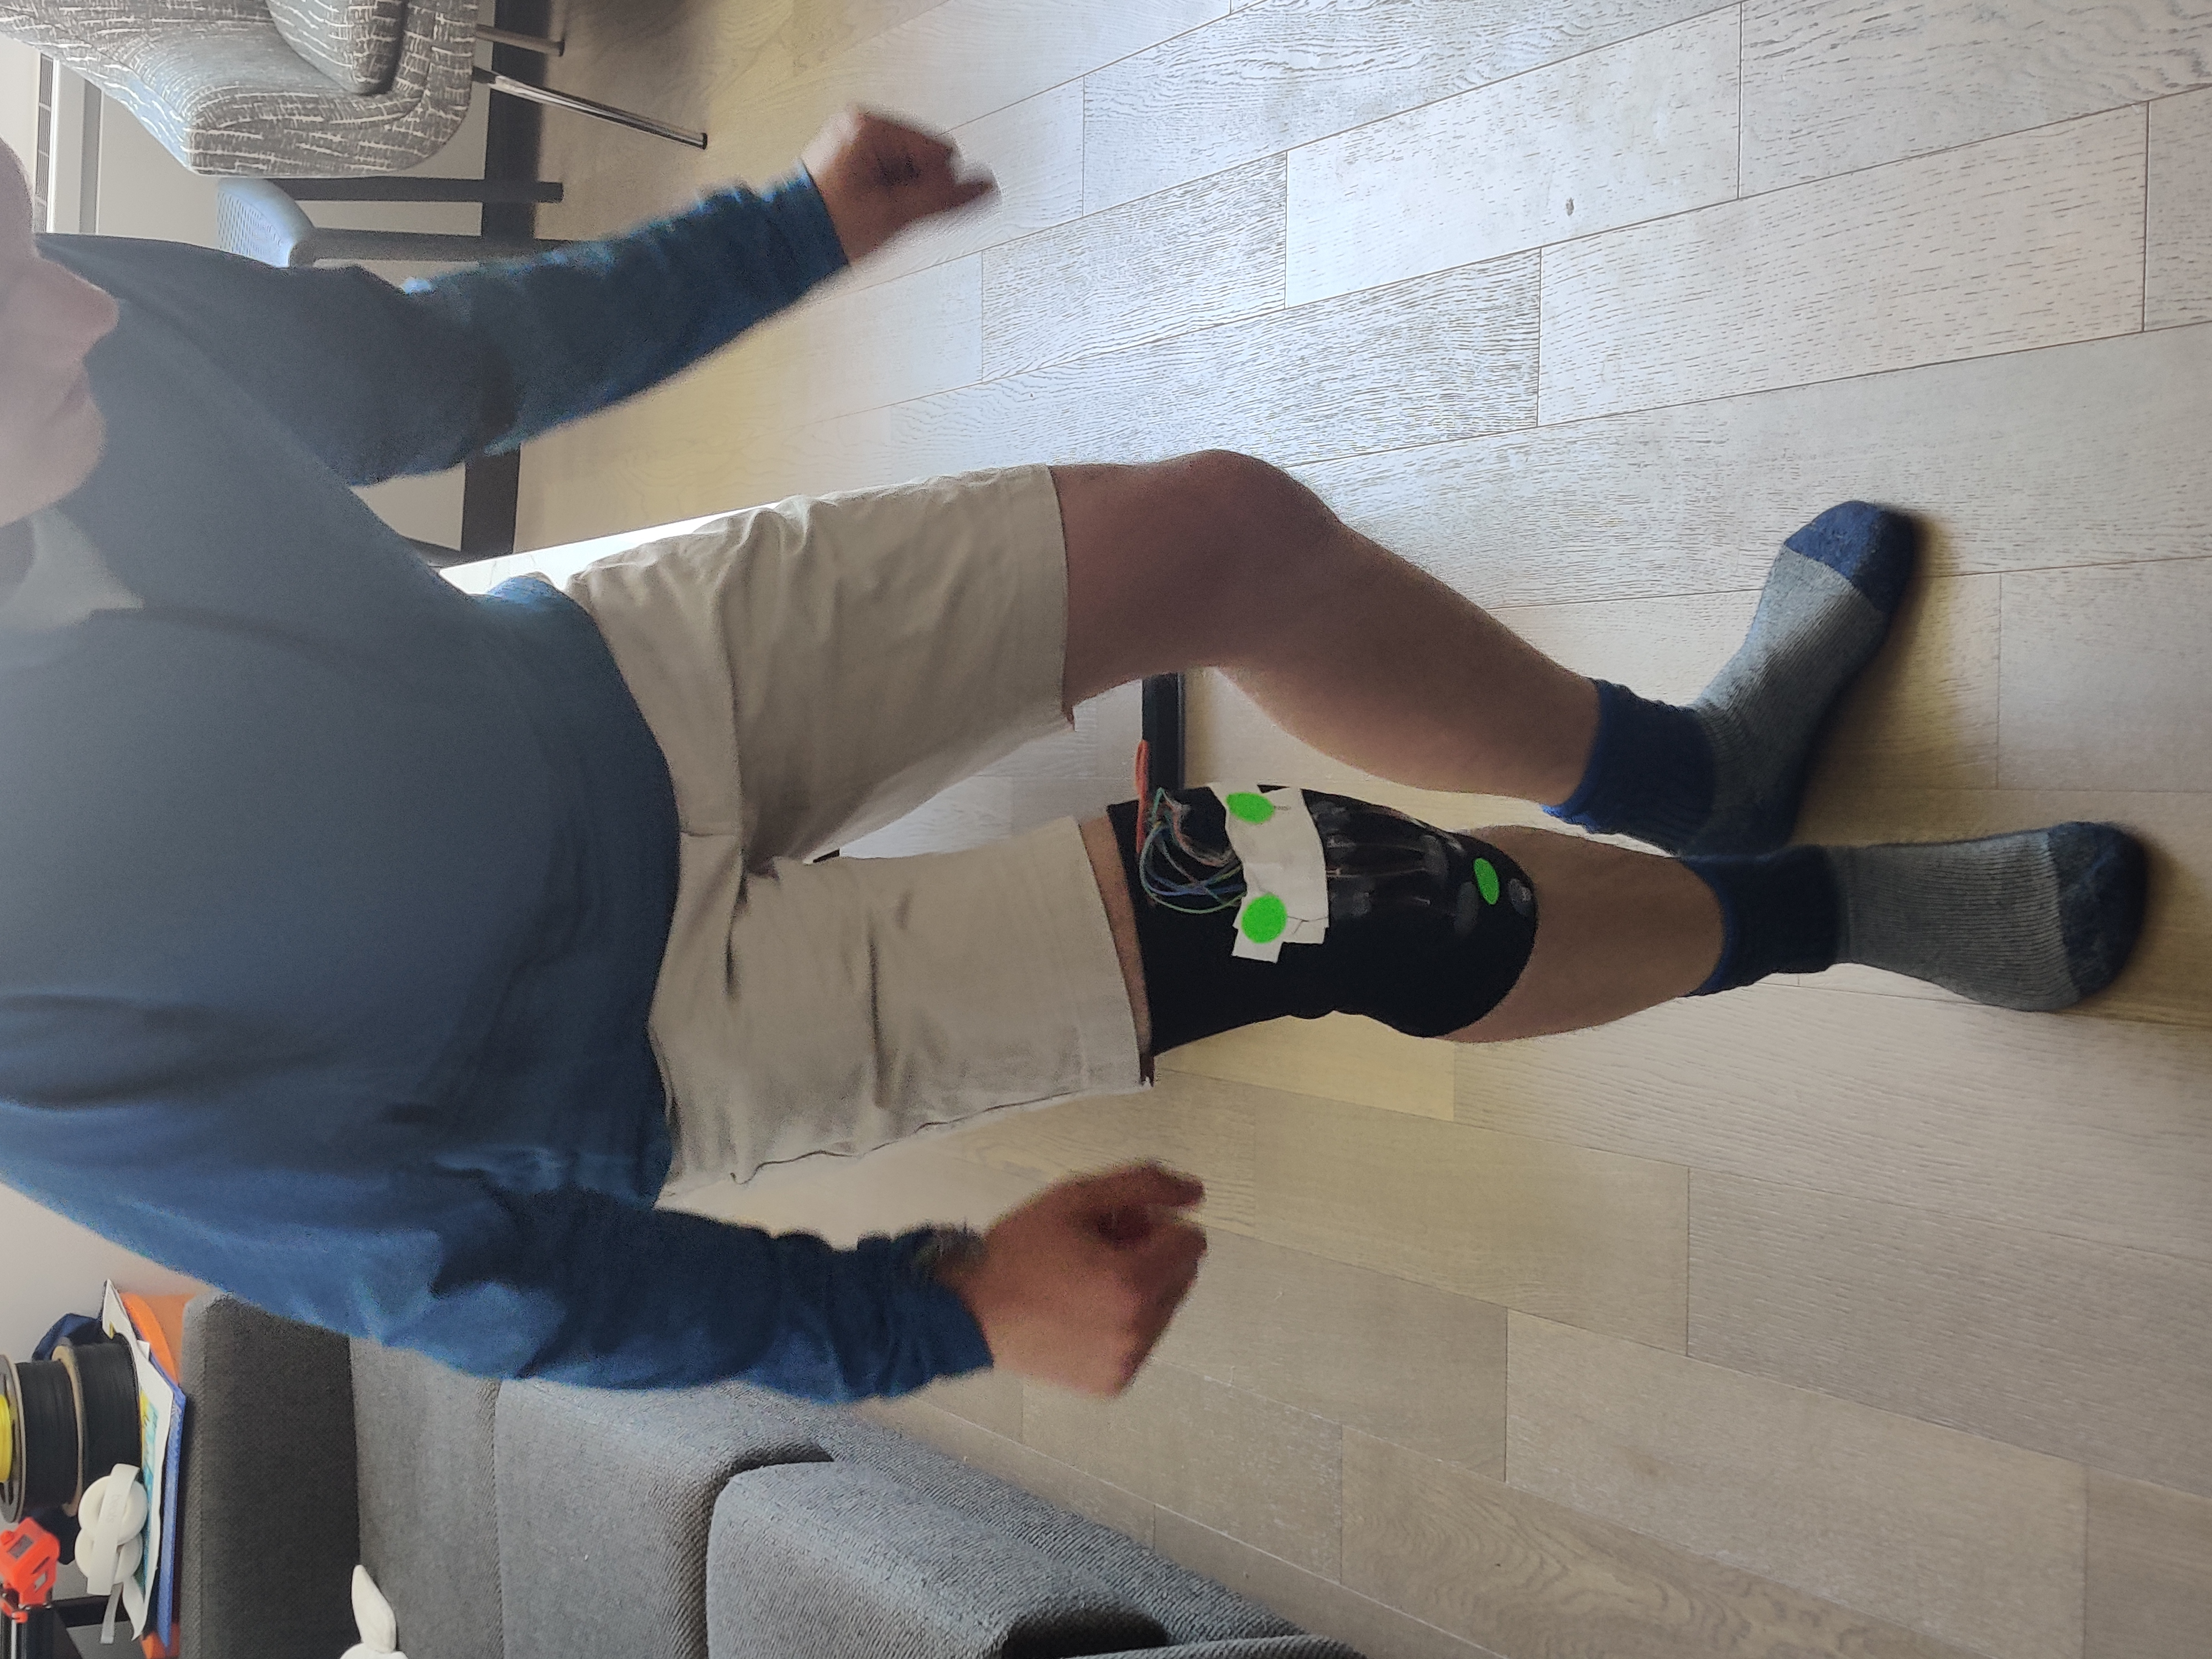
\includegraphics[width=0.65\linewidth, angle=-90]{images/jumping.jpg}
  \caption{Prototype Kneepad Jumping}
  \Description{Prototype \textit{Jump Force} kneepad, in action.}
  \label{fig:jumping_kneepad}
\end{figure}

\section{Results} \label{sec:results}

In the experiment we recorded samples from four participants over the span of two days. The participants completed the experimental procedure, as described in detail here \ref{sec:procedure}. Below are the questionnaire results from each of the participants \ref{tab:questionnaire}.

% TODO - insert table here

% see https://www.tablesgenerator.com

% how many times and for what duration the participant exercises per week, if they are involved in any sports and if so, which ones, how they would rate their athletic abilities, the longest distance they are able to run, and how high do they think they are able to jump.

\begin{table}[ht]
  \caption{Questionnaire Data}
  \label{tab:questionnaire}
  \begin{tabular}{clllll}
    \toprule
    Participant & Exercise / Week & Sports & Ability (/ 10) & Jump Distance (m) & Jump Height (m) \\
    \midrule
    1 & 4 & soccer, tennis & 6 & 2.3 & 1.1 \\
    2 & 2 & soccer & 7 & 2.5 & 0.8 \\
    3 & 3 & - & 2 & 1.6 & 1.0 \\
    4 & 4 & ultimate frisbeez soccer & 7 & 3.0 & 1.1 \\
  \bottomrule
\end{tabular}
\end{table}

After running the full data processing pipeline, I generated the below correlation matrices, grouped by participant and by sensor type \ref{tab:force_correlations}.

% TODO - insert table here

\begin{table}[ht]
  \caption{Force correlations for each participant by sensor type.}
  \label{tab:force_correlations}
  \begin{tabular}{cllllll}
    \toprule
    Participant & Avg Max Force (N) & Avg Height (m) & Flex Angle & Hall Effect Angle & Combined Angle & Acceleration \\
    \midrule
    1 & 695.3 & 1.2 & 0.753 & 0.663 & 0.742 & 0.794 \\
    2 & 628.4 & 1.1 & 0.824 & 0.645 & 0.783 & 0.843 \\
    3 & 631.3 & 0.7 & 0.731 & 0.655 & 0.717 & 0.786 \\
    4 & 734.5 & 1.6 & 0.782 & 0.629 & 0.766 & 0.812 \\
    Average & 672.4 & 1.2 & 0.773 & 0.648 & 0.752 & 0.809 \\
  \bottomrule
\end{tabular}
\end{table}

The next table shows the correlation matrices with all sensor values normalized by acceleration and jump height \ref{tab:force_correlations_normalized}.

% TODO - fix this table

\begin{table}[ht]
  \caption{Force correlations of normalized data for each participant.}
  \label{tab:force_correlations_normalized}
  \begin{tabular}{clllll}
    \toprule
    Participant & Avg Max Force (N) & Avg Height (m) & Flex Angle & Hall Effect Angle & Combined Angle \\
    \midrule
    1 & 695.3 & 1.2 & 0.862 & 0.787 & 0.870 \\
    2 & 628.4 & 1.1 & 0.898 & 0.803 & 0.904 \\
    3 & 631.3 & 0.7 & 0.785 & 0.746 & 0.778 \\
    4 & 734.5 & 1.6 & 0.855 & 0.712 & 0.868 \\
    Average & 672.4 & 1.2 & 0.850 & 0.762 & 0.855 \\
  \bottomrule
\end{tabular}
\end{table}

Looking at the first table \ref{tab:force_correlations}, the IMU average acceleration has the highest correlation with force. However, when the sensor data is normalized by dividing by the jump height and acceleration, the correlation increases to be more than the acceleration \ref{tab:force_correlations_normalized}. This shows that the angular acceleration of your knee contains useful information that further explains the characteristics of your jump, and can be used to improve an approximation of the force applied with the jump.

\section{Conclusion}

In conclusion, this experiment successfully showed, with a small sample size, that the force exerted when jumping can be accurately estimated using a low-cost sensor system. Just using an accelerometer can produce somewhat accurate results, but when combined with knee angle data from either a flex sensor matrix or hall effect sensor, can produce the results needed for a good \textit{Return to Play Protocol} test. Eliminating the need for a force plate has additional benefits. It enables anyone to easily conduct the \textit{Return to Play Protocol} test, and allows for users to save a periodic benchmark to compare against. This would be particularly useful for athletes that are in high-knee impact sports, such as running, soccer and ultimate frisbee. However, this project was relatively limited in scope due to time constraints. Any future work would need to conduct the same experiment on more participants, collect more data, and verify the results.

The data collection pipeline is done, but the user interface needs work, especially on the result display side. An important question that was not answered in this paper, is whether athletes would be willing to conduct these periodic benchmark tests, and save this data for when they get injured. Based on the number of injuries per year (see \ref{sec:introduction}), it was assumed that athletes would invest the time if they are concerned, but this would be good to verify. Finally, we would recommend that future work be focused on how to leverage camera vision to improve the accuracy of this system even further. It would be interesting to explore if there is a way to classify the type of jump (whether users are jumping from with mainly their calves or quads, for example) and how that relates to force exerted. There are many avenues for further exploration, and it is definitely an exciting space to be in, with many meaningful questions to answer.

\newpage

%%
%% The acknowledgments section is defined using the "acks" environment
%% (and NOT an unnumbered section). This ensures the proper
%% identification of the section in the article metadata, and the
%% consistent spelling of the heading.
\begin{acks}
I would like to thank Professor Alexander Adams for his invaluable help in working through the design process and feedback on the project overall. Without him this project would not have been possible.
\end{acks}

%%
%% The next two lines define the bibliography style to be used, and
%% the bibliography file.
\bibliographystyle{ACM-Reference-Format}
\bibliography{references}

%%
%% If your work has an appendix, this is the place to put it.
\appendix

\section{Source Code}

All of the source code and data can be found at the following url, under the \textit{jump\_force} folder. The GitHub repo is set to public, so anyone can access it: \url{https://github.com/jschmidtnj/ubicomp}. If more information is needed, feel free to add a pull request or write in the \textit{discussions} page in the repo.

\end{document}
\endinput
%%
%% End of file `sample-manuscript.tex'.
